\chapter{Introduction}

The introductory chapter of this work starts with a brief presentation of the main parts  and physical principles of the tokamak, a device for magnetically confine plasma. Afterwards it  explains the relation between magnetic fields and the forces generated into the tokamak geometry  as well as an introduction of control in tokamaks, which is the main topic of this thesis. This chapter closes with the thesis outline and the highlights of the carried out work. 

\section{Magnetic confinement device: the tokamak}

The tokamak is now at days the most promising configuration for a future nuclear fusion reactor and its basically a device which confines plasma through magnetic fields generated by a different set of coils positioned on an specific topology.  The tokamak is conformed by an axisymmetric torus with a large toroidal magnetic field, a moderate plasma pressure and a relatively small toroidal current also called plasma current ~\cite[Chapter~13]{Freidberg2007}. In addition to the axisymmetric torus containing the plasma there are other vital elements in the tokamak configuration ~\cite[Chapter~1]{Song2014}: \smallskip

\begin{figure}[h]
	\centering
	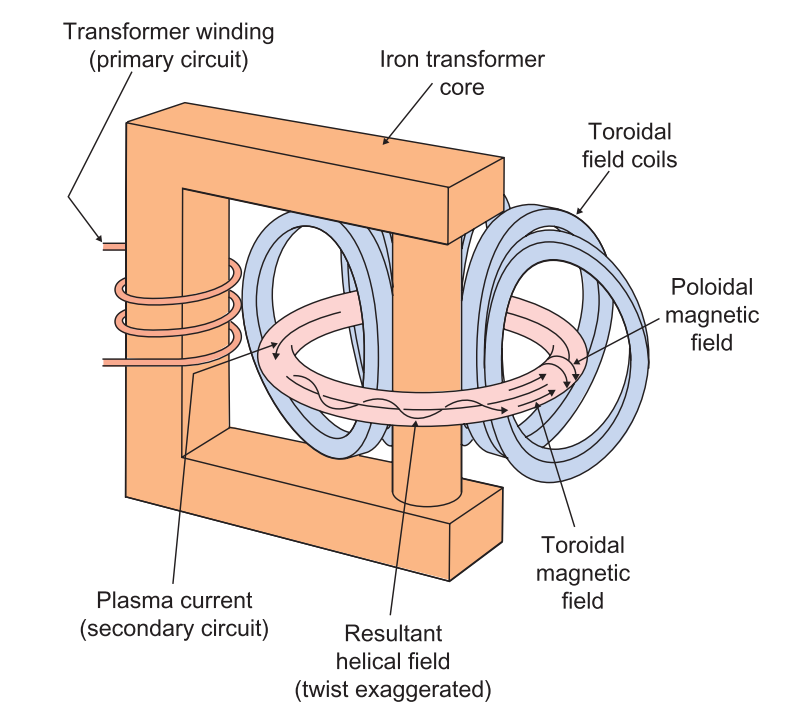
\includegraphics[width=0.8\textwidth]{Chp1/Tokamak_parts.png}
	\caption{ ~\cite{McCracken2005} \label{Tkmk_parts}}
\end{figure}

\begin{enumerate}
	\item Toroidal Field coils: Are responsible for establishing a toroidal magnetic field  and confine the plasma particles.
	\smallskip
	
	\item Poloidal Field (PF) coils : These coils generate a poloidal magnetic field  to ensure the plasma away from the wall and keep the shape and stability of the plasma.\smallskip
	
	\item Central solenoid: It acts as a transformer and its main function is to induce plasma current, where it acts as the secondary of the transformer. The plasma current creates a poloidal magnetic field additional to the one given by the PF coils. \smallskip
	
\end{enumerate}

The current stage of some actual fusion devices is described on table:



\begin{table}[]
	\centering
	\begin{tabular}{|l|c|c|c|c|}
		\hline
		\rowcolor{color2}
		\multicolumn{5}{|c|}{\textbf{Tokamak }}                                                                 \\ \hline
		\rowcolor{color1}
		Controller                 & \multicolumn{2}{c|}{eXtreme Shape Controller} & \multicolumn{2}{c|}{QST Controller}                 \\ \hline
		LCFS reconstruction method & CCS                   & CREATE                & CCS                      & CREATE                   \\ \hline
		EAST                  & China               & 0.0088                & \cellcolor[HTML]{C0C0C0} & \cellcolor[HTML]{C0C0C0} \\ \hline

JET                 & UK               & 0.0088                & \cellcolor[HTML]{C0C0C0} & \cellcolor[HTML]{C0C0C0} \\ \hline
	\end{tabular}
	\caption{ Tokamak }
	\label{Tokamak_table}
\end{table}


\section{Magnetic fields and the tokamak}

\textbf{What is a fusion plasma and why is it magnetically confined for nuclear fusion devices?}

A fusion plasma is a fully ionized gas whose behavior is dominated by long-range electric and magnetic fields. A major consequence of this behavior is that a plasma is an exceptionally good conductor of electricity, its conductivity implies that the plasma inside is shielded from DC electric fields $\bar{E}$ to a very large degree. On the other hand, DC magnetic field $\bar{B}$ can penetrate and it is this field that provides plasma confinement, hence the name "magnetic confinement" ~\cite[Chapter~6]{Freidberg2007}.\smallskip

\textbf{Why do we need magnetic fields in nuclear fusion devices ?}
\smallskip

Magnetic fields are needed to confine the hot plasma and keep it away from the machine walls.  In a generic magnetic fusion reactor the basic properties of magnetic fields require  a toroidal geometry so it can hold the plasma equilibrium ~\cite[Chapter~4]{Freidberg2007}. The properties of the magnetic fields require a toroidal geometry for confining magnetically the plasma. Trajectories of particles in the presence of magnetic fields are described by the Lorentz force equation $m \frac{d\bar{v}}{dt}=q(\bar{E}+\bar{v}\times \bar{B})$, where $\frac{d\bar{r}}{dt}=\bar{v}$, the combined perpendicular and parallel motion of a charged particle corresponds to a helical trajectory as  depicted in figure ~\ref{Helical}. If particles stream in a cylindrical device, they would collide with the wall due to the motion of the particles, a magnetic device whose lines are wrapped around  a toroidal shape  prevent free streaming end loss, making obvious why the magnetic geometry for confining the plasma has to be toroidal.\smallskip

\begin{figure}
	\centering
	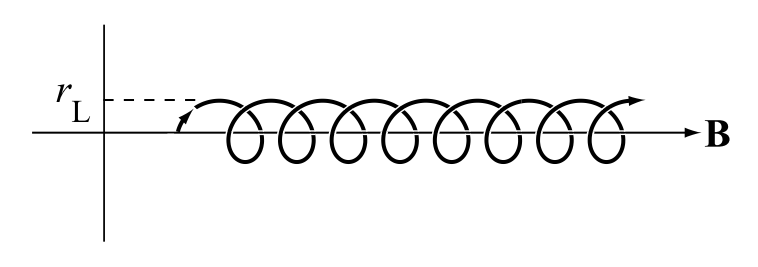
\includegraphics[width=0.525\textwidth]{Chp1/Helical_tray.png}
	\caption{  Helical trajectory of a charged particle in a uniform magnetic field ~\cite[Chapter~8]{Freidberg2007}.\label{Helical}}
\end{figure}

\section{Behind the plasma current}

Considering the drift of guiding center of a charged partice in a simple toroidal field in cylindrical coordinates $(R,\varphi,z)$. The component of the magnetic field $B_\varphi$ is the toroidal field and it decreases in the form of 1/R outward. The magnetic lines of force are circles around z axis. Particles in this  torus run fast in the toroidal direction and drift slowly in the $z$ direction as shown in figure~\ref{TDrift}, this drift is called toroidal drift. As a consequence  using only a toroidal component of magnetic field is not sufficient for confining the plasma inside a toroidal device or  tokamak  since particles drift and therefore will cause a loss of confinement ~\cite[Chapter~3]{Miyamoto2011}.\smallskip


\begin{figure}
	\centering
	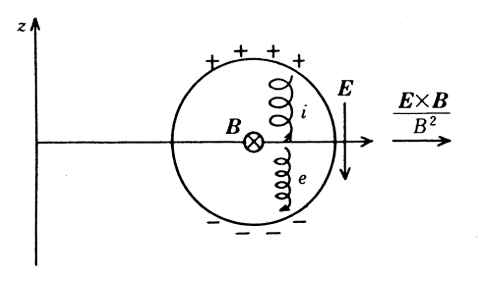
\includegraphics[width=0.55\textwidth]{Chp1/ToroidalDrift.png}
	\caption{Toroidal drift, particles drift in the vertical direction. ~\cite[Chapter~3]{Miyamoto2011} \label{TDrift}}
\end{figure}



If a current is induced in a toroidal plasma, the component of magnetic field around the magnetic axis (which is also called minor axis) is introduced. This component $B_P$ is called poloidal magnetic field and has components in $(R,z)$. The addition of this field creates magnetic lines circling the major axis of the torus, thus the particles circulate through the force lines. These lines cross a certain cross-section $P$ of the torus, each time the lines cross the plane $P$, the crossing point rotates around the minor axis by a certain angle $\iota$ which is called "rotational transform angle", this is shown in figure ~\ref{rot_angle}. The combination of toroidal and poloidal magnetic fields avoids the drift  described before originated by having an only-toroidal magnetic field by the introduction of the  rotational transform angle. The poloidal field in a tokamak is mainly produced by the induced plasma toroidal current.  \smallskip

\begin{figure}
	\centering
	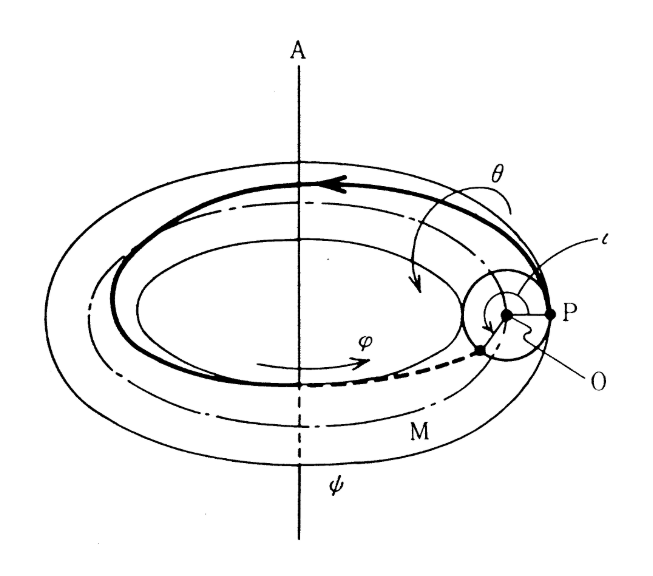
\includegraphics[width=0.655\textwidth]{Chp1/rotational_angle.png}
	\caption{Rotational transform angle $\iota$ formed when the magnetic force lines generated by the combination of toroidal and poloidal field cross the plane $P$ in different points  ~\cite[Chapter~3]{Miyamoto2011}. \label{rot_angle}}
\end{figure}

 All toroidally confined plasmas experience  outward toroidal forces along the $R$ direction, the first one is called the "hoop force" and is analogous to  the outward expansion force generated by the current flowing in a circular loop of wire, for this case this force corresponds to the toroidal current flowing in the plasma or simply called plasma current $I_p$. The second force is called "1/R force" and its name comes from the 1/R dependence of the toroidal field resulting from the toroidal geometry, the applied toroidal field $B_{\phi a}$,  where $a$ is the minor radius of the tokamak or the distance from the center of the vacuum chamber to the wall. It has a 1/R dependence which follows from integrating Ampere's law around any closed toroidal loop located between the toroidal coils and the plasma. Finally the third one is called "tire tube force" and its existence is related to the difference of plasma pressures created by the toroidal geometry ~\cite[Chapter~11]{Freidberg2007}. \smallskip 
 
Given these outward toroidal forces, somehow the  toroidal force balance must be established before the plasma hits the walls. An inwardly pointing restoring force is required and it is apply by means of the external PF coils which generate a vertical field in order to compensate the radial forces generated by the tokamak.  By choosing the magnitude and sign of the vertical field correctly, one can produce an inward restoring force to produce toroidal force balance. In order to make an analytic deviation of the toroidal force balance a simple model for the magnetic fields is used. This model consists of a toroidal plasma whose contours of constant pressure are a set of nested concentric circles $p=p(r)$, where $r$ is the minor radius coordinate as shown in figure~\ref{tor_geo}. The simplified version of the pressure and magnetic fields to be used in the determination of the toroidal force balance are:

	\begin{equation}
	\begin{aligned}
	p=&p(r)\\
	B =& \frac{R_0}{R}B_{\phi}(r) \hat{\phi} + \frac{R_0}{R}B_{\theta}(r)\hat{\theta}+B_v \hat{z}
	\end{aligned}
	\end{equation}
	
where $R_0$ is the tokamak major radius or the distance from the center of the torus to the center of the chamber (see figure ~\ref{tor_geo}) and the magnetic field $B$ is defined in toroidal coordinates ($\phi,\theta,z$) where $B_{\theta}$ is the poloidal field and $B_v$ the external vertical field generated by the PF coils. After substituting the expression for the magnetic field into the general MHD force balance equation or the so-called Grad-Shafranov equation (\cite[Chapter~6]{Miyamoto2011},~\cite[Chapter~11]{Freidberg2007},~\cite[Chpater~2]{Zohm2015}), the expression for the toroidal force balance can be obtained.
\smallskip

\begin{figure}
	\centering
	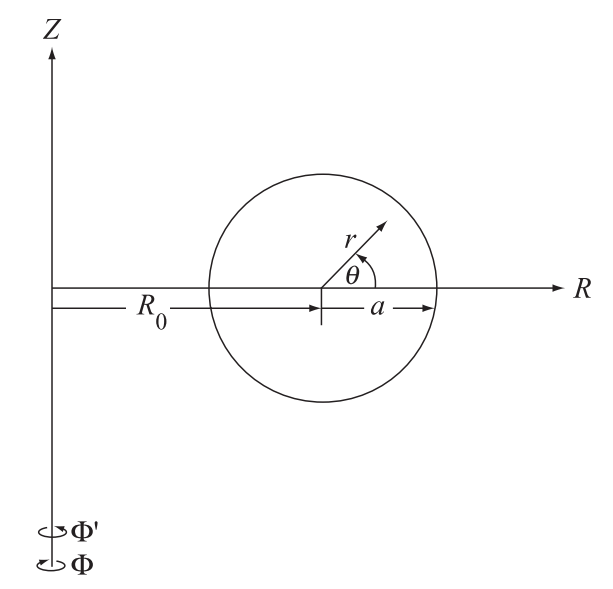
\includegraphics[width=0.6\textwidth]{Chp1/toroidal_geo.png}
	\caption{  Toroidal geometry and variables used for the calculations of the toroidal force balance and the vertical field~\cite[Chapter~11]{Freidberg2007}.\label{tor_geo}}
\end{figure}
%this is achieved by means of the application of an external vertical field.$


The toroidal force balance establishes the forces equation $F_{hoop}+ F_{1/R} + F_{tube}+ F_{v} =0$, where $F_v$ is the force generated by the external vertical field. Thus, the hoop force is given by:

\begin{equation}
F_{hoop}=2\pi^2a^2(li+le+2)~\frac{B_{\theta a}^2}{2\mu_0}
\end{equation}
 where $le$ and $li$ are the external and internal normalized inductances, $l= (L/2\pi R_0)/(\mu_0/4\pi)$. The "1/R" force is established as:
 
 \begin{equation}
 F_{1/R}=2\pi^2a^2 \left(\frac{ B_{\phi a}^2}{2\mu_0 }-\frac{\langle B_{\phi}^2 \rangle}{ 2\mu_0}\right)
 \end{equation}

where $\langle B_{\phi}^2 \rangle$ is the toroidal field average. The "tire tube" force is given by:
\begin{equation}
F_{tube}=2\pi^2a^2\langle p \rangle
\end{equation}

and finally the external vertical force is:

\begin{equation}
F_v=-2\pi^2a^2\left(\frac{2R_0 B_v B_{\theta a}}{a\mu_0}\right)
\end{equation}
 where $B_v$ is the external vertical magnetic field. Doing the combination of the 4 forces into the forces equation, the required vertical field for toroidal force balance remains:
 
 \begin{equation}
 B_v=B_{\theta a} ~\frac{a}{4R_0}\left[ \frac{2\mu_0 \langle p \rangle }{ B_{\theta a}^2} ~+~\frac{ B_{\phi a}^2 - \langle B_{\phi}^2 \rangle }{B_{\theta a}^2 } +li+le+2 \right]
 \label{force_balance}
 \end{equation}
  $B_v$ is the necessary vertical external field in order to avoid the plasma moving outwardly and touch the chamber walls, this equation will be addressed in chapter 4. In a purely vertical field, the plasma does not experience a vertical force and the vertical plasma current position is not well defined \cite[Chapter~4]{Zohm2015}. Due to the form  that the PF coils are positioned around the vessel the field produced by them is not completely vertical generating thus a radial component of  external magnetic field.  Due to Lorentz force law  the radial component of the external field  causes a vertical displacement of the plasma, this is compensated by adding another set of PF coils which generate an horizontal magnetic field. Figures ~\ref{PFcoils} show the field lines created by the vertical PF coils and its geometrical configuration surrounding the vacuum chamber. \smallskip
  
  \begin{figure}
  	\centering
  	\begin{subfigure}[b]{0.39\textwidth}
  		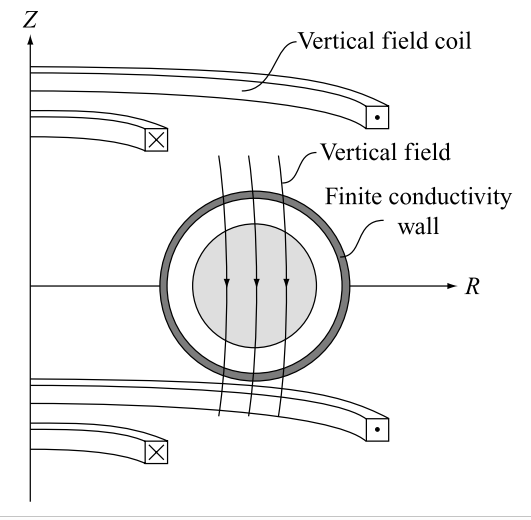
\includegraphics[width=\textwidth]{Chp1/PFcoils.png}
  		\caption{ Qualitative positioning of a set of vertical PF coils in a tokamak ~\cite[Chapter~11]{Freidberg2007}. The PF coils depicted consist of a set of quadrupole coils,  the internal coils currents are in the opposite direction to ones in the external coils. \label{} }
  	\end{subfigure}
  	~~
  	\begin{subfigure}[b]{0.39\textwidth}
  		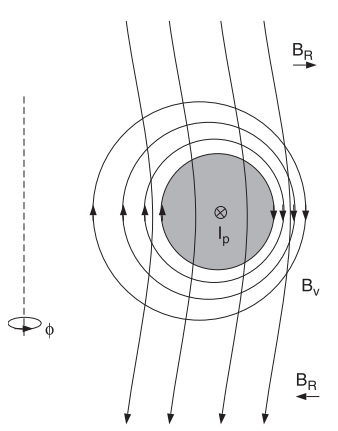
\includegraphics[width=\textwidth]{Chp1/horizontalField.png}
  		\caption{ Magnetic field lines created by the vertical PF coils with a radial field component as a result of the PF coils geometry \cite[Chapter~4]{Zohm2015}. \label{}    }
  	\end{subfigure}
  	\caption{ PF vertical coils and magnetic field lines.\label{PFcoils} }
  \end{figure}
  
  
  
\section{Plasma control in tokamaks}

Tokamaks are devices with an axisymmetric configuration with a large toroidal magnetic field and a DC toroidal current or plasma current $I_p$. Given its physical characteristics and its performance until now it is presently the leading candidate to become the world’s first fusion reactor. During the start up and subsequent approximately steady state phase of many fusion plasma discharges a toroidal current is induced in the plasma by means of transformer action with the plasma being the secondary of the transformer  ~\cite[Chapter~9]{Freidberg2007}. Sometimes the name PF coils is used to refer to  both the equilibrium field coils and the ohmic heating coils. By raising the current of the primary windings of the current transformer (ohmic heating coils), a current is induced in the plasma, which acts as the secondary winding. For example at the ISTTOK tokamak the plasma is heated by the ohmic heating coils which also generate a vertical magnetic field ~\cite[Chapter~16]{Miyamoto2011}. \smallskip

Typical operation of a tokamak discharge starts with the establishment of a large, steady, toroidal, magnetic field\footnote{Ideally, tokamaks should have superconductive toroidal coils since they do not dissipate power in steady state and require only a small amount of cooling power~\cite[Chapter~5]{Freidberg2007}.}. Next, neutral gas is injected into the vacuum chamber and often pre-ionized. The transformer induces the plasma current $I_p$ which is then ramped up to its maximum value and maintained for the “flat top” portion of the pulse~\cite[Chapter~13]{Freidberg2007}. \smallskip

Data acquisition and storage of signals in tokamaks is vitally important since the collected data us use for modeling the plasma, study instabilities and develop new codes and algorithms. Since currently tokamaks have a plasma pulsed nature of some ~ms or ~s, in the case of bigger devices, it is easy to acquire a large volume of data over short periods and archive it after the plasma discharge or even during the plasma discharge. \smallskip

Usually tokamak control tends to refer to the control of the plasma itself, while the supervisory plant control is conventional and normally uses industrial equipment. Control engineering for magnetic confined plasmas  embrace different types of techniques and used for  controlling the  physical variables existing on the device and the plasma. The tokamak control problems can be separated into two major classes: electromagnetic control and plasma kinetic control. Electromagnetic control refers to controlling the magnetic and electric fields and kinetic control refers to controlling particle feed rates and heating to modify the plasma density, temperature, pressure and current density \cite[Chapter~1]{PirontiBook}.  One of the main tasks of control engineering in the field of fusion is to maintain the plasma in certain position and shape in such way that it stays stable, follows set points and rejects possible instabilities which may occur maintaining a constant plasma current. \smallskip

Early tokamaks were quite primitive. The desired plasma parameters were obtained as a result of sets of pre-programmed power-supply or gas-valve commands, designed by trial and error, using feed forward control. As  tokamak technology began to develop and the plasma pulses duration became longer, feedback control loops were integrated to control simple parameters~\cite{Lister1999}. It is natural that one of the first parameters to be actively controlled in a tokamak was the plasma position since this would mean maintaining the hot plasma centered inside the vacuum vessel. As already explained in the previous section coupling between the plasma radial position and current control systems depend on the active PF coil system. Initially, research efforts concentrated on the radial position control of circular, vertically stable tokamak plasmas \cite[Chapter~1]{PirontiBook}. By the end of the 1970's, the advantages of forcing the tokamak plasma cross-section to be other than circular  were being proposed on the basis of theoretical studies that showed advantages regarding  an increased energy confinement time  obtained using a vertically elongated cross-section and the first plasmas with such charactersitcs where created. These elongated  plasmas are inherently unstable but this fact contributed to master the shape plasma control \cite[Chapter~1]{PirontiBook}. \smallskip



\section{Thesis outline}

The main contributions of this doctoral work  are a long  evaluation and comparison of plasma models and controllers for the  JT-60SA flat-top scenario and  a full experimental  development of the ISTTOK real-time controller and successful operation in AC mode. 

This thesis studies the properties and control applications for two tokamaks: JT-60SA and ISTTOK. These tokamaks possess physical characteristics which vary in big scale between them: the size, ISTTOK has a cross-circular section and JT-60SA is a diverted plasma, the dimension of the magnetic fields and plasma current, ISTTOK has 30 years operating and JT-60SA will start operations in late 2020, etc. Despite these facts there is a relevant reason to join the two machines in a single work: both tokamaks rely on active magnetic control applied to the PF coils in order to control the plasma position and shape. Moreover, both use active magnetic control for the plasma position,and in this work for both tokamaks control and modeling approaches relying in the same concepts are applied.   \smallskip

ISTTOK has been used for young researchers training with relevant 
emphasis in several PhD thesis. The present thesis is one more contribution to this endeavor where the concepts learned and applied to the simulation work of JT-60SA  could be confirmed in a practical sense in ISTTOK. \smallskip

This work is divided in 5 chapters being this chapter the Introduction.\smallskip

$\bullet$ Chapter 2 explores the plasma control systems implemented in different tokamaks around the world and addresses some important theoretical concepts to be applied in the further chapters.\smallskip

$\bullet$ Chapter 3 addresses JT-60SA operation, its theoretical modeling and assessments for the shape and plasma current control.\smallskip

$\bullet$ Chapter 4 presents the overall picture of ISTTOK tokamak: the geometry, the actuators and diagnostics. Following, the novel  implemented  reconstruction of the plasma current centroid position is addressed.\smallskip

$\bullet$ Chapter 5  presents the experimental control results in ISTTOK after the implementation of two different control algorithms in the device. \smallskip

The research done in this work is important and needed because it delves into topics crucial for tokamak operation. It assesses control techniques for what will be the biggest operating tokamak before ITER (JT-60SA) and implements novelty algorithms in a small tokamak that probably would have not  existed on the ISTTOK tokamak without the latest technology advances. The main objectives of this thesis are to encompass the implementation of novel  plasma position and shape controllers for two different devices demonstrating that despite the size or characteristics of a tokamak it relies in the same physics principles and control engineering tools.\smallskip 
